\documentclass{standalone}
\usepackage{tikz}
\usetikzlibrary{shapes}
\begin{document}
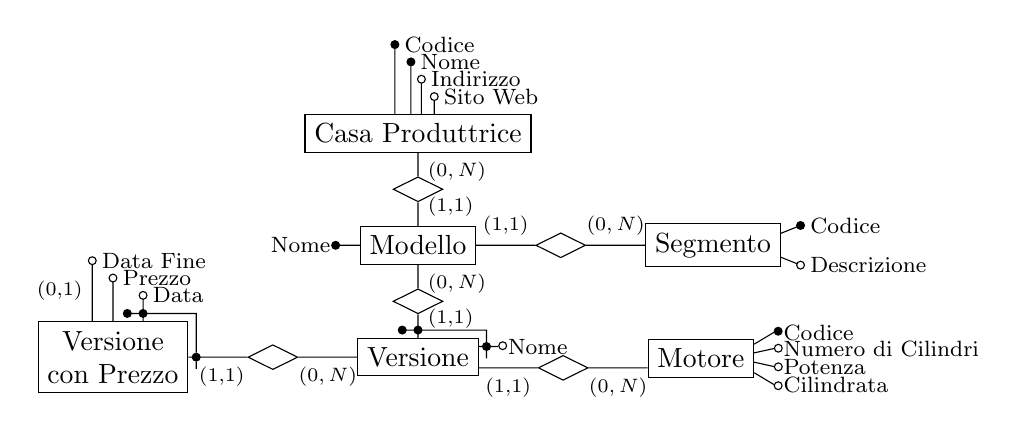
\begin{tikzpicture}
    \draw

    % casa produttrice
    (0,0)node[draw, rectangle](casa){Casa Produttrice}
    (casa.140)--++(0,0.88)node[draw, circle, inner sep=1pt, fill=black]{}node[right]{\footnotesize Codice}
    (casa.110)--++(0,0.66)node[draw, circle, inner sep=1pt, fill=black]{}node[right]{\footnotesize Nome}
    (casa.80)--++(0,0.44)node[draw, circle, inner sep=1pt, fill=white]{}node[right]{\footnotesize Indirizzo}
    (casa.50)--++(0,0.22)node[draw, circle, inner sep=1pt, fill=white]{}node[right]{\footnotesize Sito Web}

    % modello
    (casa.270)node[below right]{\scriptsize $(0,N)$}--++(0,-0.3)node[draw, diamond, shape aspect=2, inner sep=3pt, anchor=90](r1){}
    (r1.270)--++(0,-0.3)node[above right]{\scriptsize (1,1)}node[draw, rectangle, anchor=90](modello){Modello}
    (modello.180)--++(-0.25,0)node[draw, circle, inner sep=1pt,anchor=0, fill=black]{}node[left]{\footnotesize Nome}

    % segmento
    (modello.0)--++(0.75,0)node[midway, above]{\scriptsize (1,1)}node[draw, diamond, shape aspect=2, inner sep=3pt, anchor=180](r3){}
    (r3.0)--++(0.75,0)node[midway, above]{\scriptsize $(0,N)$}node[draw, rectangle, anchor=180](segmento){Segmento}
    (segmento.10)--++(0.25,0.1)node[draw, circle, inner sep=1pt, fill=black]{}node[right]{\footnotesize Codice}
    (segmento.350)--++(0.25,-0.1)node[draw, circle, inner sep=1pt, fill=white]{}node[right]{\footnotesize Descrizione}

    % versione
    (modello.270)node[below right]{\scriptsize $(0,N)$}--++(0,-0.3)node[draw, diamond, shape aspect=2, inner sep=3pt, anchor=90](r2){}
    (r2.270)--++(0,-0.2)node[draw, circle, inner sep=1pt,fill=black](a){}--++(0,-0.1)node[above right]{\scriptsize (1,1)}node[draw, rectangle, anchor=90](versione){Versione}
    (versione.10)--++(0.1,0)node[draw, circle, inner sep=1pt, fill=black](b){}--++(0.15,0)node[draw, circle, inner sep=1pt,anchor=190]{}node[right]{\footnotesize Nome}

    (a)++(-0.2,0)node[draw, circle, inner sep=1pt, fill=black](){}-|(b)--++(0,-0.15)

    % motore
    (versione.350)--++(0.75,0)node[midway, below]{\scriptsize (1,1)}node[draw, diamond, shape aspect=2, inner sep=3pt, anchor=180](r3){}
    (r3.0)--++(0.75,0)node[midway, below]{\scriptsize $(0,N)$}node[draw, rectangle, anchor=190](motore){Motore}
    (motore.15)--++(0.25,0.15)node[draw, circle, inner sep=1pt,anchor=195, fill=black]{}node[right]{\footnotesize Codice}
    (motore.6)--++(0.25,0.055)node[draw, circle, inner sep=1pt,anchor=184]{}node[right]{\footnotesize Numero di Cilindri}
    (motore.356)--++(0.25,-0.055)node[draw, circle, inner sep=1pt,anchor=176]{}node[right]{\footnotesize Potenza}
    (motore.345)--++(0.25,-0.15)node[draw, circle, inner sep=1pt,anchor=165]{}node[right]{\footnotesize Cilindrata}
    
    % versione con prezzo 
    (versione.180)--++(-0.75,0)node[midway, below]{\scriptsize $(0,N)$}node[draw, diamond, shape aspect=2, inner sep=3pt, anchor=0](r3){}
    (r3.180)--++(-0.65,0)node[midway, below]{\scriptsize (1,1)}node[draw, circle, inner sep=1pt, fill=black](b){}--++(-0.1,0)node[draw, rectangle, anchor=0, align=center](versione){Versione\\con Prezzo}
    (versione.120)--++(0,0.77)node[midway, left]{\scriptsize (0,1)}node[draw, circle, inner sep=1pt, fill=white]{}node[right]{\footnotesize Data Fine}
    (versione.90)--++(0,0.55)node[draw, circle, inner sep=1pt, fill=white]{}node[right]{\footnotesize Prezzo}
    (versione.50)--++(0,0.1)node[draw, circle, inner sep=1pt, fill=black](a){}--++(0,0.23)node[draw, circle, inner sep=1pt, fill=white]{}node[right]{\footnotesize Data}

    (a)++(-0.2,0)node[draw, circle, inner sep=1pt, fill=black](){}-|(b)--++(0,-0.15)


    ;    
\end{tikzpicture}
\end{document}